\documentclass{article}
\usepackage[utf8x]{inputenc}
\usepackage{ucs}
\usepackage{amsmath} 
\usepackage{amsfonts}
\usepackage{upgreek}
\usepackage[english,russian]{babel}
\usepackage{graphicx}
\usepackage{float}
\usepackage{textcomp}
\usepackage{hyperref}
\usepackage{geometry}
  \geometry{left=2cm}
  \geometry{right=1.5cm}
  \geometry{top=1cm}
  \geometry{bottom=2cm}
\usepackage{tikz}
\usepackage{ccaption}
\usepackage{multicol}

\usepackage{listings}
%\setlength{\columnsep}{1.5cm}
%\setlength{\columnseprule}{0.2pt}


\begin{document}
\pagenumbering{gobble}

\lstset{
  language=C,                % choose the language of the code
  basicstyle=\linespread{1.1}\ttfamily,
  columns=fixed,
  fontadjust=true,
  basewidth=0.5em,
  keywordstyle=\color{blue}\bfseries,
  commentstyle=\color{gray},
  stringstyle=\ttfamily\color{orange!50!black},
  showstringspaces=false,
  %numbers=false,                   % where to put the line-numbers
  numbersep=5pt,
  numberstyle=\tiny\color{black},
  numberfirstline=true,
  stepnumber=1,                   % the step between two line-numbers.        
  numbersep=10pt,                  % how far the line-numbers are from the code
  backgroundcolor=\color{white},  % choose the background color. You must add \usepackage{color}
  showstringspaces=false,         % underline spaces within strings
  captionpos=b,                   % sets the caption-position to bottom
  breaklines=true,                % sets automatic line breaking
  breakatwhitespace=true,         % sets if automatic breaks should only happen at whitespace
  xleftmargin=.2in,
  extendedchars=\true,
  keepspaces = true,
}
\lstset{literate=%
   *{0}{{{\color{red!20!violet}0}}}1
    {1}{{{\color{red!20!violet}1}}}1
    {2}{{{\color{red!20!violet}2}}}1
    {3}{{{\color{red!20!violet}3}}}1
    {4}{{{\color{red!20!violet}4}}}1
    {5}{{{\color{red!20!violet}5}}}1
    {6}{{{\color{red!20!violet}6}}}1
    {7}{{{\color{red!20!violet}7}}}1
    {8}{{{\color{red!20!violet}8}}}1
    {9}{{{\color{red!20!violet}9}}}1
}

\section*{Хеш-таблицы}



\begin{figure}[H]
\centerline{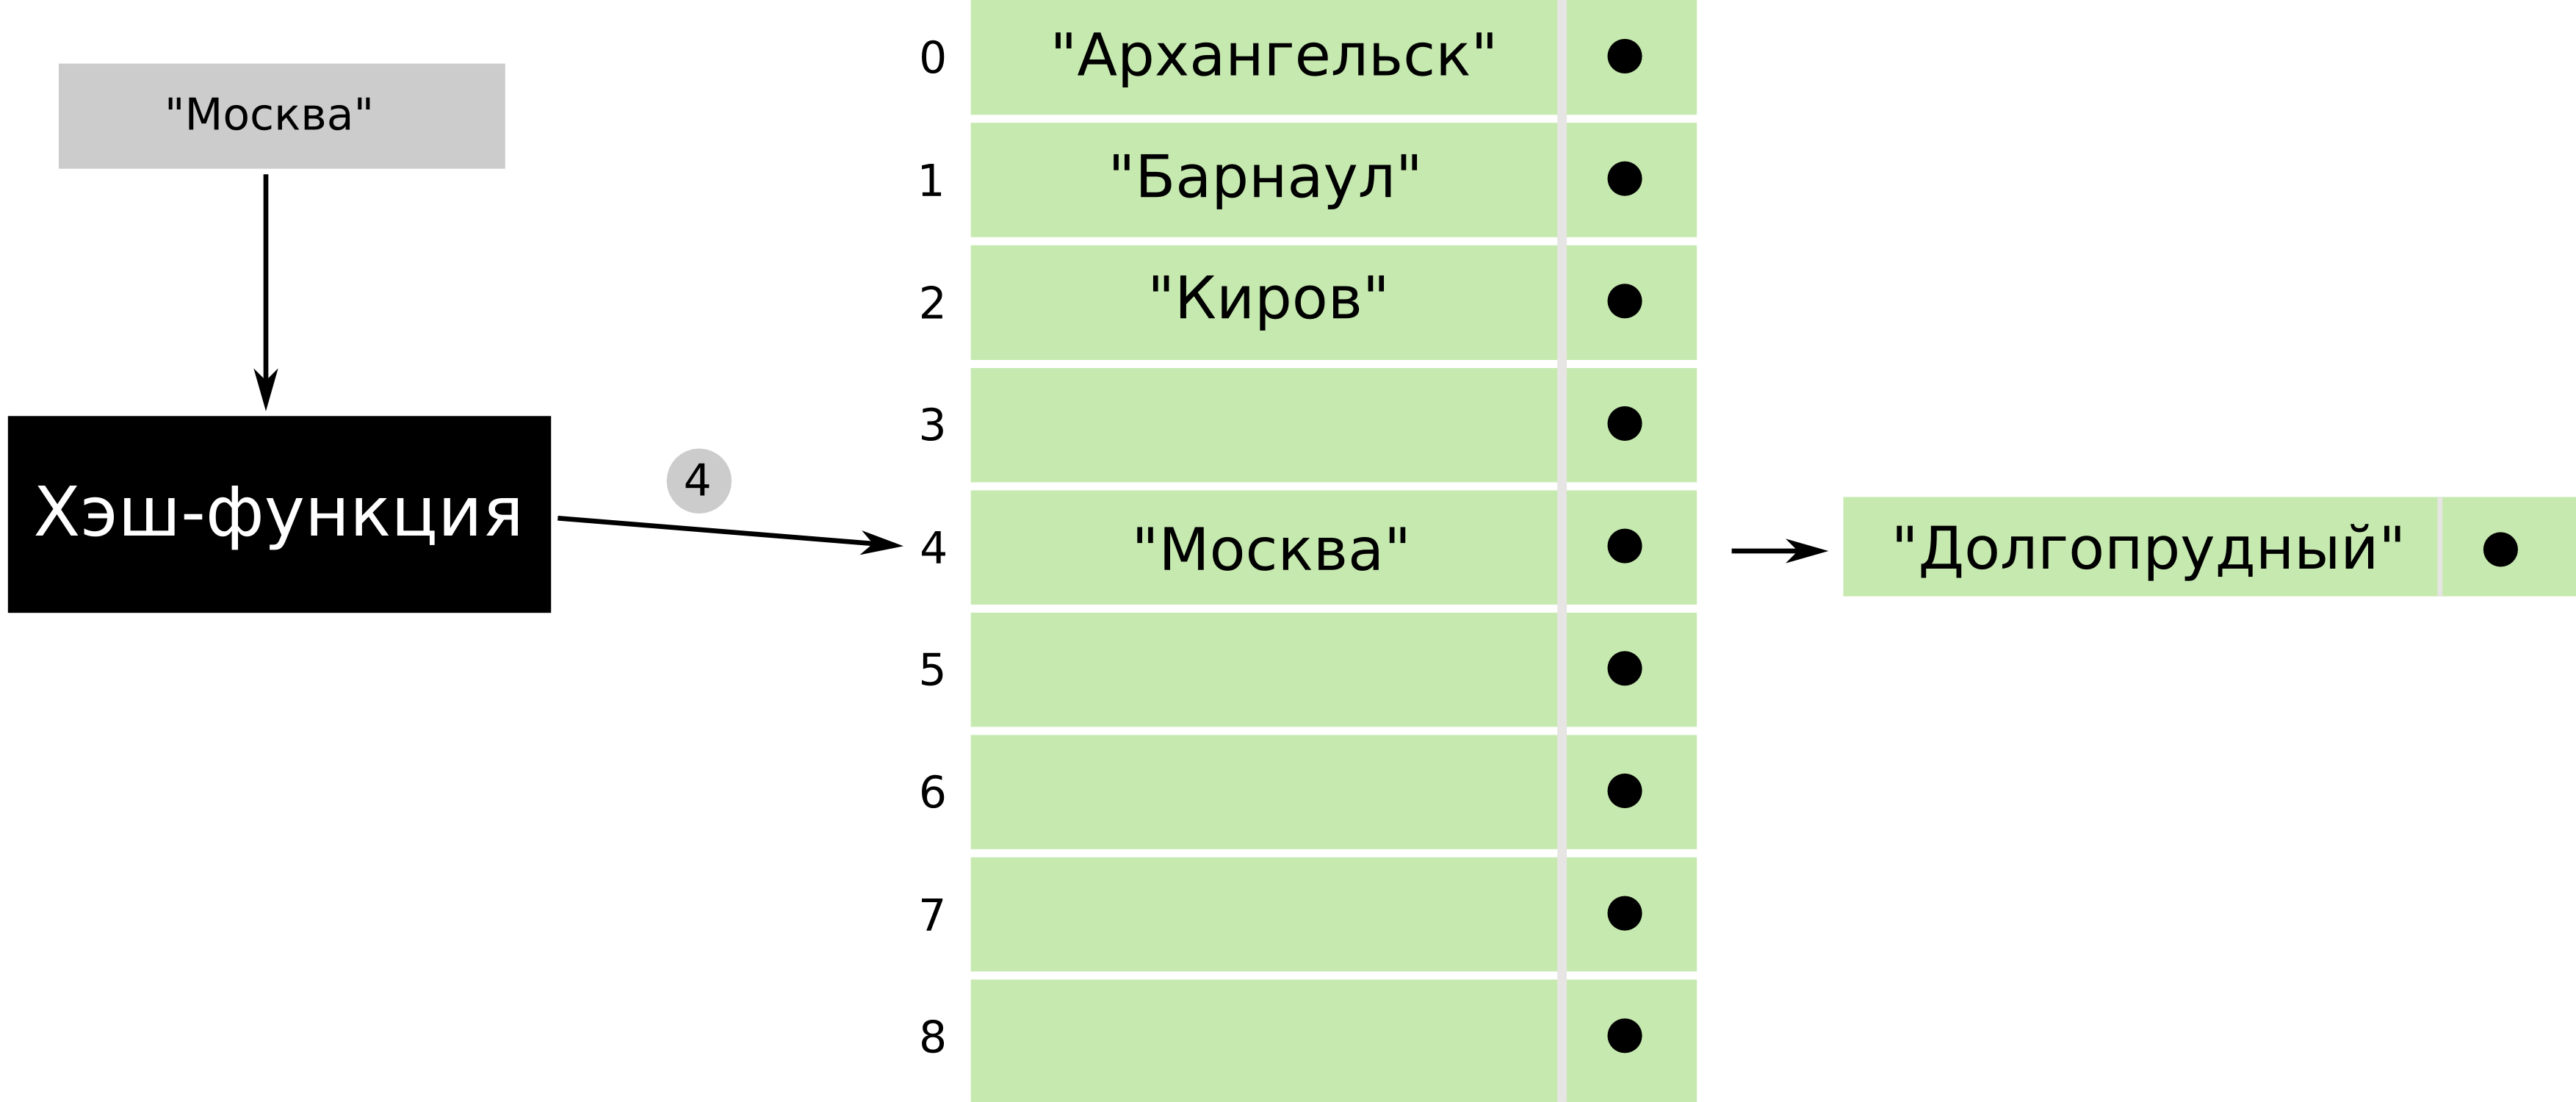
\includegraphics[width=0.7\linewidth]{hash_8.png}}
\end{figure}

\begin{multicols}{2}
\begin{lstlisting}
#define INITIAL_SIZE (1024)
#define GROWTH_FACTOR (2)
#define MAX_LOAD_FACTOR (1)

struct node 
{
    struct node* next;
    char* key;
    char* value;
};
typedef struct node Node;

struct hashtable 
{
    /* Размер таблицы */
    int size;      
    /* Количество элементов в таблице */     
    int n;              
    struct node** table;
};
typedef struct hashtable Hashtable;



// Функция, которая добавляет элемент в хеш-таблицу
Hashtable* hashtable_create(int size)
{
    int i;
    Hashtable* ht = 
         malloc(sizeof(Hashtable));

    ht->size = size;
    ht->n = 0;
    ht->table = malloc(sizeof(struct node*)*ht->size);

    for(i = 0; i < ht->size; i++) 
        ht->table[i] = 0;

    return ht;
}
\end{lstlisting}
\end{multicols}{2}


\subsection*{Задачи}
\begin{enumerate}
\item Написать функцию \texttt{void hashtable\_insert(Hashtable* ht, char* key, char* value)}, которая добавляет элемент в хештаблицу. Для этого вам понадобится простейшая хеш-функция:
\begin{lstlisting}
unsigned long hash_function(const char *s)
{
    unsigned long h = 0;
    for(unsigned char* p = s; *p; p++)
        h = h * 97 + *p;
    return h;
}
\end{lstlisting}

\item Написать функцию \texttt{void print\_hashtable(Hashtable* ht)}, которая будет печатать все элементы хеш-таблицы.

\item Используйте функции из предыдущих двух задач, чтобы добавить в хештаблицу 10 элементов. Напечатайте эту хещ-таблицу.

\item Написать функцию \texttt{char* search\_hashtable(Hashtable* ht, char* key)}, которая будет искать элемент в хеш-таблице по ключу.

\item Написать функцию \texttt{void grow\_hashtable(Hashtable* ht)}, которая будет увеличивать хеш-таблицу в\\ GROWTH\_FACTOR раз.

\item Считать данные из файла \texttt{citiydescriptions.txt} в хеш-таблицу. Добавьте в хеш-таблицу большое количество элементов и проследите как меняется её размер. 

\end{enumerate}
\end{document}